\chapter{The Renormalization Group}
\section[The Wilsonian Renormalization Group]{The Wilsonian Renormalization Group\footnote{P \& S, Ch 12.1}}
We will study influence of UV fluctuations more explicitly using UV cutoff $\Lambda$. It is difficult for gauge theories, but more intuitive for $\phi^4$.

Consider path integral with field vanishes in momentum space,
\begin{align*}
   Z[J] &= \int [\D \phi] \exp{i\int \dd[4]{x} (\lag + \phi J)} \\
        &= \prod_k \int \dd{\phi(k)}  \exp{i\int \dd[4]{x} (\lag + \phi J)}
\end{align*} 
We would like to separate out integration over modes with $|k| \leq \Lambda$. It is difficult in Minkowski space, since Minkowski "scalar product" is not positive semi-definite. So first perform Wick rotation to Euclidean space, where momentum cutoff $\Lambda$ is well defined. Euclidean path integral
\begin{align}
   \eval{Z_E[J]}_{J=0} &= \int [\D \phi]_\Lambda \exp{-\int \dd[d]{x_E} \left(\frac{1}{2} ( \partial \phi)^2 + \frac{1}{2} m^2 \phi^2 + \frac{\lambda}{4!}\phi^4 \right)}
\end{align}
Drop the subscript $E$ from now on. $m$ and $\lambda$ are bare parameters, there are no counter-terms yet. Dimension $d$ to keep discussion general.

Idea is to lower the cutoff $\Lambda$ somewhat, from $\Lambda \rightarrow b \Lambda$, with b a small positive number $ 0 < b < 1$. 
\paragraph{Define} \underline{low- and high-momentum modes} 
\begin{align}
   \tilde{\phi}(k) &= \begin{cases} \phi(k) & |k| \leq b \Lambda  \\ 0 &  |k| > b\Lambda \end{cases} \\
   \hat{\phi}(k) &= \begin{cases} 0 & |k| \leq b \Lambda \\ \phi(k) & b \Lambda < |k| \leq \Lambda \end{cases}
\end{align}
so that field can be decomposed into low-momentum modes and high-momentum modes.
\begin{align}
   \phi(k) = \tilde{\phi}(k) + \hat{\phi}(k) 
\end{align}
Rename low-momentum mode $\tilde{\phi}(k) = \phi(k)$.

In the path integral $[\D \phi]_{\Lambda} = [\D \phi]_{b \Lambda} [\D \hat{\phi}]$ and substitute $\phi \mapsto \phi + \hat{\phi}$ in the Lagrangian.
\begin{align*}
   Z &= \int [\D \phi]_{b \Lambda} \int [\D \hat{\phi}] \exp{ - \int \dd[d]{x} \left[\frac{1}{2} (\partial \phi + \partial \hat{\phi})^2 + \frac{m^2}{2}(\phi + \hat{\phi})^2 + \frac{\lambda}{4!} (\phi + \hat{\phi})^4 \right] } \\
     &=  \int [\D \phi]_{b \Lambda} \exp{- \int \dd[d]{x} \lag [\phi]} \int [\D \hat{\phi}] \exp{ - \int \dd[d]{x} \left[ \frac{1}{2} (\partial \hat{\phi})^2 + \frac{m^2}{2} \hat{\phi}^2 + \lambda \left(\frac{1}{6} \phi^3 \hat{\phi} + \frac{1}{4} \phi^2 \hat{\phi}^2 + \frac{1}{6} \phi \hat{\phi}^3 + \frac{1}{4!} \hat{\phi}^4 \right) \right]}
\end{align*}
Note that terms of order $\phi\hat{\phi}$ vanish! They would contribute to propagator-type terms, not have disjoint momentum support (different Fourier components orthogonal!)

Interaction terms of the form (double line for high momentum modes, single line for low momentum modes)
\begin{align*}
   \feynmandiagram[small, layered layout]{
      i1 -- v-- f1;
      i2 -- v-- f2;
   };\quad 
   \feynmandiagram[small, layered layout]{
      i1 -- v--[double] f1;
      i2 -- v-- f2;
   };\quad 
   \feynmandiagram[small, layered layout]{
      i1 -- v--[double] f1;
      i2 -- v--[double] f2;
   };\quad 
   \feynmandiagram[small, layered layout]{
      i1 --[double] v--[double] f1;
      i2 -- v--[double] f2;
   };\quad 
   \feynmandiagram[small, layered layout]{
      i1 --[double] v--[double] f1;
      i2 --[double] v--[double] f2;
   };
\end{align*}

After $\int \D \hat{\phi}$ path integral is carried out, the generating function should look like
\begin{align*}
   Z \stackrel{!}{=} \int [\D \phi]_{b \Lambda} \euler^{-\int \dd[d]{x} \lag_\text{eff}(\phi)}
\end{align*}
Now $\lag_\text{eff}$ only involves Fourier components with $|k| \leq b \Lambda$.

How does $\lag_\text{eff}$ look like?
\begin{align}
   \lag_\text{eff} = \lag(\phi) + \text{corrections}
\end{align}
The corrections are in order of $\lambda$. The correction terms compensate for the removal of high-momentum Fourier components/fluctuations in $\hat{\phi}$.

We are interested in large-ish cutoffs $\Lambda^2 \gg m^2$. Treat $m^2$ and $\lambda$ terms in the $\D \hat{\phi}$ path integral as perturbations. Leading propagator comes from
\begin{align*}
   \int \dd[d]{x} \lag_0 &= \int \dd[d]{x} \frac{1}{2} (\partial \hat{\phi})^2 \\
                         &= \int \frac{\dd[d]{k}}{(2\pi)^d} \frac{1}{2} \hat{\phi}^*(k) k^2 \hat{\phi}(k)
\end{align*}

The contraction is similar to a normal propagator 
\begin{align}
   \bcontraction{}{\hat{\phi}}{(k)}{\hat{\phi}} \hat{\phi} (k) \hat{\phi} (p) = \frac{\int \D \hat{\phi} \hat{\phi}(k) \hat{\phi} (p) \euler^{-\int \dd[d]{x} \lag}}{\int \D \hat{\phi} \euler^{-\int \dd[d]{x}\lag_0 }} \notag \\
   = \frac{1}{k^2} (2\pi)^d \delta^{(d)}(p + k) \hat{\theta}(k)  \label{math:phiphi}
   \shortintertext{where}
   \hat{\theta}(k) = \begin{cases} 1 & b \Lambda < |k| \leq \Lambda \\ 0 & \text{otherwise} \end{cases} \notag
\end{align}

Perturbations in $m^2$ and $\lambda$ are calculated expanding the exponential, using Wick's theorem with propagator from above. What corrections in $\lag_\text{eff}$ will the $\hat{\phi}$ field generate?

\paragraph{Tree level diagrams} 
Diagram with $\phi^3 \bcontraction{}{\hat{\phi}}{\phi^3}{\hat{\phi}} \hat{\phi} \phi^3 \hat{\phi}$
\begin{align*}
   \feynmandiagram[baseline=(v1.base), small, horizontal=v1 to v2, layered layout]{
      {i1[particle=\(p_1\)], i2[particle=\(p_2\)], i3[particle=\(p_3\)]} -- v1 --[double] v2 -- {f1[particle=\(p_1\)], f2[particle=\(p_2\)], f3[particle=\(p_3\)]};
   };
   \sim \frac{\lambda^2}{(p_1 + p_2+ p_3)^2} \hat{\theta} (p_1 + p_2 + p_3)
\end{align*}
does not contribute for $p_1, p_2, p_3 \ll \Lambda^2$. Similarly other tree-level diagrams won't contribute.

Consider $p_i = 0$ (external) for now!

\paragraph{Single $\hat{\phi}$ loop}
\begin{align*}
   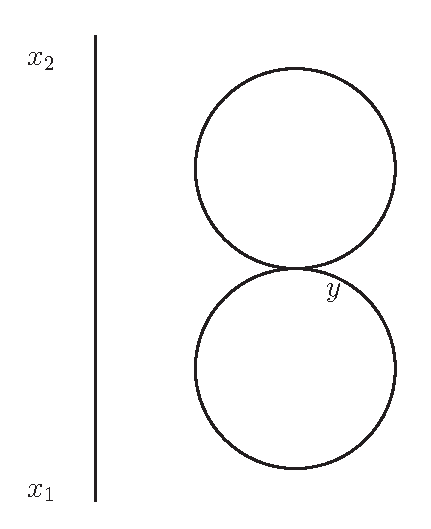
\includegraphics[width=0.8\linewidth]{./RG/1.eps}
\end{align*}

Calculate $(1)$ explicitly using equation (\ref{math:phiphi})
\begin{align*}
   (1) = -\frac{\lambda}{4}  \int \dd[d]{x} \phi^2 \bcontraction{}{\hat{\phi}}{}{\hat{\phi}} \hat{\phi} \hat{\phi} &=: - \frac{1}{2}\int \frac{\dd[d]{k_1}}{(2\pi)^d} \Delta m^2 \phi(k_1) \phi(-k_1)  \\
\end{align*}
in which 
\begin{align*}
   \Delta m^2 &= \frac{\lambda}{2} \int_{b \Lambda < |k| \leq \Lambda} \frac{\dd[d]{k}}{(2\pi)^d} \frac{1}{k^2} \\
              &= \frac{\lambda}{2} \frac{\Omega_d}{(2\pi)^d} \int_{b \Lambda}^\Lambda \dd{k} k^{d-3} \\
              &= \frac{\lambda}{(4\pi)^{d/2}} \frac{1}{\Gamma (d/2)} \frac{\Lambda^{d-2}}{d-2} (1- b^{d-2})
   \shortintertext{with $n$ dimensional solid angle $\Omega_d = 2 \pi^{d/2} / \Gamma(d/2)$. In $d=4$}
   \Delta m^2 &= \frac{\lambda}{16 \pi^2} \frac{\Lambda^2}{2} (1-b^2)
\end{align*}
 Remember $b < 1$ so $\Delta m^2 > 1$.

Second diagram give $- \frac{\Delta \lambda}{4!} \phi^4$ in effective Lagrangian. Setting external momenta to zero
\begin{align*}
   \Delta \lambda &= - 4! \frac{2}{2!} \left(\frac{\lambda}{4}\right)^2 \int \frac{\dd[d]{k}}{(2\pi)^d} \left( \frac{1}{k^2} \right)^2  \\
                  &= - \frac{3}{2} \lambda^2 \frac{2}{(4\pi)^{d/2} \Gamma(d/2)} \int_{b \Lambda}^{\Lambda} \dd{k} k^{d-5} \\
                  &= \frac{-3 \lambda^2}{(4\pi)^{d/2} \Gamma(d/2)} \frac{\Lambda^{d-4}}{d-4} (1-b^{d-4})  \\
                  &= - \frac{3 \lambda^2}{16 \pi^2} \ln( \frac{1}{b})
\end{align*}
It's negative since $0 < b < 1$!

If we set external momenta $p_i \neq 0$: Taylor expand in $p_i$,  it will generate interactions terms $(\partial \phi)^2 \phi^2$, $(\partial \phi)^4$, $\dots$.

Third diagram generates term $\sim \lambda^3 \phi^6$ (in $d=4$, $\propto \frac{\lambda^3 \phi^6}{\Lambda^2}$). Higher dimensional, non-renormalizable interactions are generated! We will see soon why it is not a real problem.

\paragraph{Comments}
\begin{itemize}
   \item Everything is finite, although being cutoff-dependent
   \item Is loop expansion $\frac{\lambda + \Delta \lambda}{4!} \phi^4$ valid?
      \begin{align*}
         \lambda + \Delta \lambda = \lambda \bigg[ 1- \underbrace{\frac{3\lambda}{16 \pi^2} \ln(1/b)}_{\ll 1} \bigg]
      \end{align*}
      Higher order ($N$ loops) will scale like $\lambda (\frac{\lambda}{16\pi^2} \ln(1/b))^N$. 
      \begin{align*}
         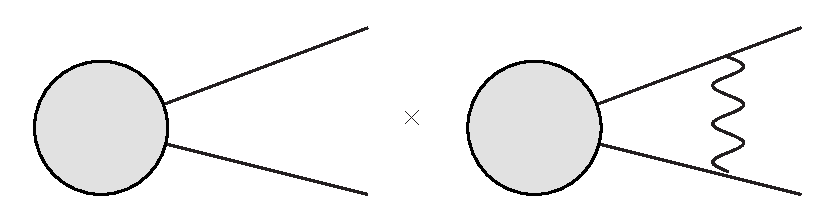
\includegraphics[width=0.4\linewidth]{./RG/2.eps} 
      \end{align*}
      It is even smaller corrections.
\end{itemize}

More careful comparison of $\lag $ and $ \lag_\text{eff}$
\begin{align*}
   Z &= \int [\D \phi]_{b \Lambda} \euler^{- \int \dd[d]{x} \lag_\eff} \\
   \lag_\text{eff} &= \frac{1}{2} (1 + \Delta Z) (\partial \phi)^2 + \frac{1}{2} (m^2 + \Delta m^2) \phi^2 + \frac{1}{4!} (\lambda + \Delta \lambda) \phi^4 + \Delta C ((\partial \phi)^2)^2 + \Delta \tilde{C} \phi^2 (\partial \phi)^2 + \Delta D \phi^6 + \dots
\end{align*}

Now rescale distances and momenta $k' = k / b$ or $x' = xb$. $k'$ in integrated up to $\Lambda$ (original cutoff).
\begin{align*}
   \int \dd[d]{x} \lag_\eff &= \int \dd[d]{x'} b^{-d} \bigg[ \frac{1}{2} (1+\Delta z) b^2 (\partial' \phi)^2 + \frac{1}{2} (m^2 + \Delta m^2)\phi^2 \\
      &+ \frac{1}{4!} (\lambda + \Delta \lambda) \phi^4 + \Delta C b^4 (\partial \phi)^4 + \tilde{\Delta C}b^2 (\partial' \phi)^2 \phi^2 + \Delta D \phi^6 + \dots \bigg]
\end{align*}
Now rescale the fields  
\begin{align*}
  \phi' = \sqrt{b^{2-d} (1+ \Delta Z)} \phi 
\end{align*}
to obtain canonical kinetic term
\begin{align*}
      \int \dd[d]{x} \lag_\eff &= \int \dd[d]{x'} \left[ \frac{1}{2} (\partial' \phi')^2 + \frac{1}{2} m'^2 \phi'^2 + \frac{1}{4!} \lambda' \phi'^4 + C' (\partial' \phi')^4 + \tilde{C}' (\partial' \phi')^2 \phi'^2 + D' \phi'^6 \right]
\end{align*}
with the scaled variables
\begin{align*}
   m'^2 &= \frac{m^2 + \Delta m^2}{b^2(1+\Delta Z)} \\
   \lambda' &= \frac{\lambda + \Delta \lambda}{b^{4-d} (1+ \Delta Z)^2} \\
   C' &= b^d \frac{C+ \Delta C}{(1+\Delta Z)^2} \\
   \tilde{C}' &= b^{d-2} \frac{\tilde{C} + \Delta \tilde{C}}{(1+\Delta Z)^2} \\
   D' &= b^{2d-6} \frac{D+ \Delta D}{(1+\Delta Z)^3}
\end{align*}
Even if we had $C = \tilde{C} = D = 0$ initially, it would apply as well.

So combination of integrating out degree of freedom and rescaling leads to transformation of $\lag$ (with identical $Llamba$). $\lag$ characterized by set of coupling constants 
\begin{align*}
  (m^2, \lambda, C, \tilde{C}, D, \dots) \mapsto (m'^2, \lambda', C', \tilde{C}', D', \dots) 
\end{align*}

This operation can be repeated, make it infinitesimal $ b \mapsto 1 - db$, so that it's continuous. Transformation in space of all possible Lagrangians.

Study trajectory or flows leads to Renormalization Group. It is not really a group, rather a semi-group, as transformation of "integrating-out" high-momentum degree of freedom is not invertible.

Two possible ways to perform calculations of correlation functions for $|p_i| \ll \Lambda$ 
\begin{itemize}
   \item use original $\lag$, high-momentum fluctuations in loops
   \item use $\lag_\eff$ high-momentum fluctuations have been absorbed in new coupling constants. Already at tree-level. Essentially it is effective field theory.
\end{itemize}

\paragraph{Renormalization Group (RG) in Detail}
Consider $\lag$ near the free theory $m^2 = \lambda =C = \tilde{C} = D = \dots = 0$
\begin{align*}
   \lag_0 = \frac{1}{2} (\partial \phi)^2
\end{align*}
$\lag_0$ is unchanged under the RG flow. It is fixed point.

Near $\lag_0$, only consider terms \underline{linear} in perturbation. Neglect $\Delta m^2 (\propto \lambda), \Delta \lambda (\propto \lambda^2), \Delta Z (\propto \lambda^2), \Delta C, \Delta \tilde{C} (\propto \lambda^2), \Delta D (\propto \lambda^3)$. Then simply have 
\begin{align*}
   m'^2 &= m^2 b^{-2} \\
   \lambda' &= \lambda b^{d-4} \\
   \tilde{C}' &= \tilde{C} b^{d-2} \\
   C' &= C b^d \\
   D' &= D b^{2d-6}
\end{align*}

Since $0 < b < 1$, behaviours are classified as following
\begin{itemize}
   \item \underline{relevant} term grows with RG, 
   \item \underline{marginal} term in $d=4$ unchanged  (higher orders unimportant)
   \item \underline{irrelevant} term diminished in RG flow
\end{itemize}

This can actually be seen directly from dimensional analysis. Operator with $N$ fields $\phi$ and $M$ derivatives scales as 
\begin{align*}
   C'_{N, M} &= b^{N(d/2 - 1) + M - d} C_{N, M} \\
             &= b^{d_{N, M} - d} C_{N, M}
\end{align*}
with $d_{N,M}$ mass dimension of the operator.

Note: relevant/marginal/irrelevant terms correspond to super-renormalizable/renormalizable/non-renormalizable interactions.

One can understand evolution of couplings near a fixed point from dimensional analysis! Near fixed point, arbitrary complicated $\lag$ reduces to a finite number of renormalizable term! (Only near fixed point!)

Illustrate RG flow for $\phi^4$ in 3 cases
\begin{itemize}
   \item \underline{$d > 4$} only mass term is relevant, everything else irrelevant. Only $m^2$ grows, since $m'^2 = m^2 b^{-2n}$ after $n$ iterations. Ultimately $m'^2 \sim \Lambda^2$. Integrate complete momentum range between $\Lambda$ and the effective mass $m'$.
   \item \underline{$d=4$} marginal $\lambda$? Go back to the full transformation including non-linear terms.
      \begin{align*}
         \lambda' = \frac{\lambda + \Delta \lambda}{b^{4-d} (1+\Delta Z)^2} = \lambda - \frac{3\lambda^2}{16\pi^2} \ln(1/b) + \order{\lambda^3}
      \end{align*}
      $\lambda$ slowly decreases as high-momentum modes are integrated out. Coupling goes to zero $\phi^4$ becomes non-interacting in $d=4$.lambda
   \item \underline{$d < 4$} $\lambda$ is relevant! Coupling grows. Non-linear effects are important. 
      \begin{align*}
         \lambda' = b^{d-4} \left[ \lambda = \frac{3\lambda^2}{(4\pi)^{d/2}} \frac{1}{\Gamma(d/2)} \frac{b^{d-4} - 1}{4-d} \Lambda^{d-4} \right]
      \end{align*}
      There is a second fixed point, besides a trivial one $\lambda = 0$.
      \begin{align*}
         \lambda = \frac{4-d}{3} (4\pi)^{d/2} \Gamma(d/2) (\Lambda b)^{4-d} > 0
      \end{align*}
      where the non-linear effects compensate the rescaling!
\end{itemize}
\begin{align*}
   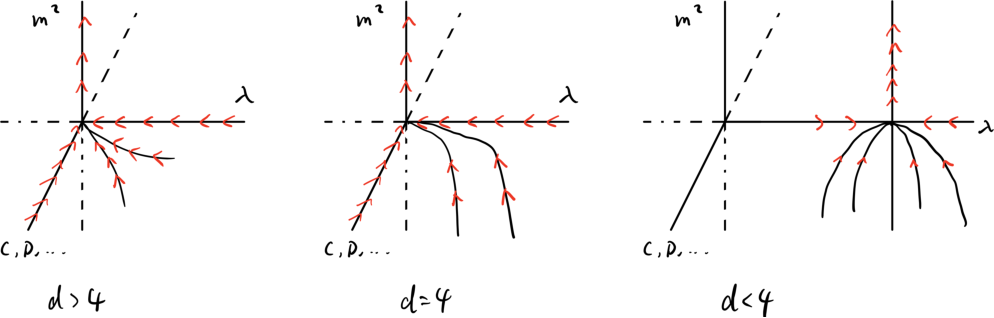
\includegraphics[width=0.8\linewidth]{./RG/RGFlow.pdf}
\end{align*}

\paragraph{Remarks}
\begin{itemize}
   \item for $d<4$ but "close", the new fixed point will be "close" to the free fixed point. Then perturbation theory still make sense. Could have strongly-coupled theories as a fixed point. More difficult, study exactly solvable models.
   \item $m^2 d^2$ in $\phi^4$ always relevant, diverges quickly, naturally $m \mapsto \Lambda$.Problems for theories with elementary scales (Higgs in Standard Model)
\end{itemize}

%%%%%%%%%%%%%%%%%%%%%%%%%%%%%%%%%%%%%%%%%%%%%%%%%%%%%%%%%%%%%%%%%
% Lecture date: 19-12-11
%%%%%%%%%%%%%%%%%%%%%%%%%%%%%%%%%%%%%%%%%%%%%%%%%%%%%%%%%%%%%%%%%

\section{Callan-Symanzik Equation}
We want to avoid technically complicated calculations with cutoffs (violate [gauge] symmetries!). Looking for a method to extract RG information from \underline{renormalized} Green's functions (limit $\Lambda \rightarrow \infty$ already taken). Cannot extract RG from $\Lambda$-dependence any more use dependence on renormalization scale $\mu$ instead!

\paragraph{$\phi^4$-theory near the critical point $m=0$}
Renormalization conditions so far, on-shell, $s=t=u=\frac{4}{3}m^2$ for $4$-point function, are problematic in the massless case. Use arbitrary (unphysical) space-like reference point $-\mu^2$. Then the two- and four-point functions are
\begin{enumerate}
   \item $\Sigma_{1\text{PI}}(p^2 = -\mu^2) = 0$,
   \item $\dv{p^2} \eval{\Sigma_{1\text{PI}}}_{p^2 = -\mu^2} = 0$,
   \item \feynmandiagram[layered layout, inline=(v.base)]{x1 -- v[blob] -- x2; x3--v--x4;}; $=-i\lambda$ at $s = (p_1+p_2)^2 = -\mu^2$, $t = -\mu^2$, $u=-\mu^2$.
\end{enumerate}
Call $\mu$ \underline{renormalization scale}.

Consequence of first two
\begin{align}
   \braket{0 | \phi(p) \phi(-p) | 0} = \eval{\frac{i}{p^2}}_{p^2 = -\mu^2} 
\end{align}
in terms of the bare field $\phi_0 = \sqrt{Z}\phi$
\begin{align}
   \braket{0 | \phi_0(p) \phi_0(-p) | 0} = \eval{\frac{iZ}{p^2}}_{p^2 = -\mu^2}
\end{align}
Do renormalized perturbation theory as before, adjusting the counterterms to the conditions above.

Note that renormalization scale $\mu$ is arbitrary; one could have chosen different value for $\mu$!

Green's functions for bare and renormalized fields
\begin{align*}
   G_{\text{base}}^{(n)} &= \braket{0 | T \phi_0 (x_1) \dots \phi_0(x_n) | 0 } \\
   G_{\text{ren}}^{(n)} &= \braket{0 | T \phi (x_1) \dots \phi(x_n) | 0 } \\
   \phi &= Z^{-1/2} \phi_0
\end{align*}
Then we have the relation
\begin{align}
   G_\text{ren}^{(n)} &= Z^{-n/2} G_\text{bare}^{(n)}
\end{align}

The 1PI vertex functions have $n$ external legs amputated.
\begin{align}
   \Gamma_\text{ren}^{(n)} = Z^{n/2} \Gamma_\text{bare}^{(n)}
\end{align}

Now shift the renormalization scale $\mu \mapsto \mu + \dd{\mu}$. Shift couplings to obtain the same physics
\begin{align*}
   \lambda \mapsto \lambda + \dd{\lambda} \\
   Z \mapsto Z + \dd{Z} \\
   [m \mapsto m + \dd{m} ] 
\end{align*}
while the bare quantities $\lambda_0, [m_0] $ remain unchanged.

\begin{align}
   \Gamma_\text{ren}^{(n)}(x_1, \dots, x_n, \lambda + \dd{\lambda}, [m + \dd{m}], \mu + \dd{\mu}) &= (Z+ \dd{Z})^{n/2} \Gamma_\text{bare}^{(n)}(x_1,\dots, x_n, \lambda_0, [m_0,] (\Lambda))
\end{align}
The infinitesimal changes are
\begin{align*}
   \dd{\Gamma}_\text{ren}^{(n)} &= \pdv{\Gamma_\text{ren}^{(n)}}{\mu} \dd{\mu} + \pdv{\Gamma^{(n)}_\text{ren}}{\lambda} \dd{\lambda} \left( + \pdv{\Gamma_\text{ren}^{(n)}}{m} \dd{m} \right) \\
                                &= \frac{n}{2} Z^{n/2-1} \dd{Z} (Z+ \dd{Z})^{n/2} \Gamma_\text{bare}^{(n)}(x_1,\dots, x_n, \lambda_0, [m_0,] (\Lambda))
\end{align*}
Thus
\begin{align*}
   \mu \pdv{\Gamma_\text{bare}^{(n)}}{\mu} &= 0 \\
   \mu \pdv{\Gamma_\text{ren}^{(n)}}{\mu} + \underbrace{ \mu \pdv{\lambda}{\mu}  }_{\beta} \pdv{\Gamma_\text{ren}^{(n)}}{\lambda} \Bigg[ + \underbrace{\mu \pdv{m}{\mu}}_{m \gamma_m} \pdv{\Gamma_\text{ren}^{(n)}}{m} \Bigg] &= \underbrace{\frac{n}{2} \frac{\mu}{Z} \pdv{Z}{\mu}}_{n \gamma} \underbrace{Z^{n/2} \Gamma_\text{bare}^{(n)}}_{\Gamma_\text{ren}^{(n)}}
\end{align*}

\underline{Callan-Symanzik Equation}
\begin{align}
   \left[ \mu \pdv{\mu} + \beta \pdv{\lambda} \left( + m \gamma_m \pdv{m} \right) - n \gamma \right] \Gamma_\text{ren}^{(n)} = 0
\end{align}
for Green's function $G_\text{ren}^{(n)}$ there is a sign change $+n\gamma$.

Per definition $\beta$ and $\gamma$ are independent of $n$. Since $\Gamma^{(n)}_\text{ren}$ is used, they are independent of cutoff $\Lambda$. For dimensional reasons, also independent of $\mu$ (in the massless case $m=0$!). $\beta$ and $\gamma$ are only functions of the dimensionless coupling constant $\lambda$! 

Compute $\beta$ and $\lambda$ in loop expansion (dimensional regularization and $\overline{\text{MS}}$) in $\phi^4$; $2$- and $4$-functions must satisfy CS-equation.
\paragraph{Tree level}
\begin{align*}
   i \Gamma_\text{tree}^{(2)} = i p^2 \\
   i \Gamma_\text{tree}^{(4)} = -i \lambda
\end{align*}
There is no $\mu$-dependence, $\beta= \gamma=0$ at tree level

\paragraph{One-loop}
\begin{align*}
   i \Gamma_\text{one-loop}^{(2)} &= i (p^2 - \Sigma(p^2))  \\
                                  &= \dots \\
                                  %TODO: diagram
                                  &= ip^2 - \frac{i\lambda \mu^{4-d}}{2} \underbrace{\int \frac{\dd[d]{q}}{(2\pi)^d} \frac{i}{q^2}}_{=0} - \delta_m^{(1)} + ip^2 \delta_Z^{(1)}
\end{align*}
If it is massive theory, the loop integral is $\sim m^2$. So the renormalization condition is fulfilled for $\delta_m^{(1)} = 0$, $\delta_Z^{(1)} = 0$, then
\begin{align}
   i\Gamma_\text{one-loop}^{(2)} = i \Gamma_\text{tree}^{(2)} = i p^2
\end{align}

See result from last term
\begin{align*}
   i \eval{\Gamma^{(4)}_\text{one-loop}}_{s = t=u=-\mu^2} &= -i\lambda - \frac{3i\lambda^2 \mu^{4-d} }{16\pi^2} \Bigg[ \frac{1}{d-4} + \frac{1}{2} \Bigg( \gamma_E - \ln(4\pi) + \underbrace{\int_0^1 \ln(x(1-x))}_{=-2} \Bigg) \Bigg] - i \delta_\lambda \\
   &\stackrel{!}{=} -i \lambda
\end{align*}

\begin{align}
   \delta_\lambda = - \frac{3\lambda^2}{16\pi^2} \mu^{4-d} \left[ \frac{1}{d-4} + \frac{1}{2} \left( \gamma_E - \ln(4\pi) \right) - 1\right]
\end{align}

Then the fully renormalized result is
\begin{align}
   i\Gamma_\text{one-loop}^{(4)}(s,t,u) &= -i\lambda - \frac{i\lambda^2}{32\pi^2} \mu^{4-d} \sum_{q^2 = s, t, u} \left[ \int \dd{x} \ln(\frac{-q^2 x(1-x)}{\mu^2}) + 2 \right] \notag \\
                                        &\stackrel{d=4}{=} -i\lambda - \frac{i\lambda^2}{32\pi^2} \sum_{q^2 = s, t, u} \left[ \int \dd{x} \ln(\frac{-q^2 x(1-x)}{\mu^2}) + 2 \right]
\end{align}

Note on the convergence of the perturbative series: corrections can be large if $\lambda \ll 1$, but $\ln(\frac{q^2}{\mu^2}) \gg 1$. Choose $\mu^2$ of the order of the typical momentum scale of the process. So large logarithm. 

Conversion to different process with different momenta $q'^2 \neq q^2$ need CS-equation.

Now evaluate CS equations
\begin{align*}
   i\Gamma_\text{one-loop}^{(2)} = ip^2 \\
   \left[ \mu \pdv{\mu} + \beta \pdv{\lambda} - n\gamma \right] p^2 = 0
\end{align*}
Thus 
\begin{align}
   \gamma = 0
\end{align}
at one-loop level.

\begin{align*}
   \left[ \mu \pdv{\mu} + \beta \pdv{\lambda} - n \gamma \right] \Gamma_\text{one-loop}^{(n)} = 0\\
   \left[ \mu \pdv{\mu} + \beta \pdv{\lambda} \right] \left[ - \lambda - \frac{\lambda^2}{32\pi^2} \left( 6 + \sum_{q^2 = s,t,u} \int_0^1 \dd{x} \ln \frac{-q^2 x (1-x)}{\mu^2} \right) \right]  = 0 \\
   \mu \left[ 0 - \frac{\lambda^2}{32\pi^2} \left(- \frac{6}{\mu} \right) \right] + \beta ( - 1 +\order{\lambda}) = \frac{3\lambda^2}{16\pi^2} - \beta(1+\order{\lambda}) = 0
\end{align*}
Thus
\begin{align}
   \beta = \frac{3\lambda^2}{16\pi^2} + \order{\lambda^3} 
\end{align}

Can we obtain this (expression for $\beta$) in an easier way? Yes! $\beta$ is determined by the $\mu$-dependence of the counterterm:
\begin{align}
   \mu \pdv{\mu} \delta_\lambda^{(1)} &= \mu \pdv{\mu} \left( - \frac{3\lambda^2}{16 \pi^2} \mu^{4-d} \left[ \frac{1}{d-4} + \dots \right] \right) \\
   \shortintertext{$\mu^{4-d} = 1 + (4-d)\ln(\mu)$}
   &= \frac{3\lambda^2}{16\pi^2} = \beta
\end{align}
It only works at one-loop, scheme dependence at higher loop orders.

\paragraph{The meaning of $\beta$ and $\gamma$}
\begin{align*}
   \beta = \mu \pdv{\mu} \lambda \\
   \dd{\lambda} = \beta(\lambda) \frac{\dd{\mu}}{\mu}
\end{align*}
It characterises rate of change in renormalized coupling for fixed bare coupling $\lambda_0$.  Associate $\lambda(\mu)$ with coupling $\lambda'$ of the Wilsonian RG: $\beta$ is rate of RG flow for $\lambda$
\begin{itemize}
   \item $\beta > 0$ coupling grows  at large momenta and shrinks at small momenta
   \item $\beta < 0$ the opposite
\end{itemize}

\begin{align}
   \gamma(\lambda) = \frac{1}{2} \frac{\mu}{Z} \pdv{Z}{\mu} = \frac{1}{2} \mu \pdv{\mu} \ln(Z)
\end{align}
is the rate of change in field strength rescaling.

\paragraph{CS Equation for QED with $m_e = 0$}
\begin{align*}
   \left[\mu \pdv{\mu} + \beta(e) \pdv{e} - n\gamma_2(e) - m\gamma_3(e) \right] \Gamma_\text{ren}^{(n,m)} = 0
\end{align*}
with $n$ number of electron fields and $m$ number of photon fields. 
\begin{align*}
   \beta (e) &= \mu \pdv{\mu} e = \frac{e^3}{12\pi^2} > 0 \\
   \gamma_2 (e) &= \frac{\mu}{2} \pdv{\mu} \ln(Z_2) = \frac{e^2}{16\pi^2} \\
   \gamma_3(e) &= \frac{\mu}{2} \pdv{\mu} \ln(Z_3) = \frac{e^2}{12\pi^2}
\end{align*}

\section{RG, Scaling of $\Gamma$ and the Running Coupling}
We will study the behaviour under rescaling of \underline{external momenta}
\begin{align}
   \Gamma_\text{ren}^{(n)} \left( \left\{ p_i \right\}; m, \lambda, \mu \right) \mapsto  \Gamma_\text{ren}^{(n)} \left( s \left\{ p_i \right\}; m, \lambda, \mu \right)
\end{align}

First rescale all dimensionfull quantities
\begin{align}
   \Gamma_\text{ren}^{(n)} \left( s\left\{ p_i \right\}; m, \lambda, \mu \right) = s^{4-n} \Gamma_\text{ren}^{(n)} \left( \left\{ p_i \right\}; m, \lambda, \mu \right)
\end{align}
according to mass dimensional of $\Gamma^{(n)}$ from dimensional analysis. For example $\Gamma^{(2)} = p^2 - m^2$, $\Gamma^{(4)} = - \lambda$

Expand around $s=1$: $s = 1+\dd{s}$, so 
\begin{align*}
   p'_i = (1+\dd{s}) p_i \\
   m' = (1+\dd{s})m \\
   \mu' = (1+\dd{s})\mu
\end{align*}

\begin{align}
   \Gamma_\text{ren}^{(n)} \left( \left\{ p'_i \right\}; m', \lambda, \mu' \right) = \left[ 1+(4-n)\dd{s} \right]  \Gamma_\text{ren}^{(n)} \left( \left\{ p_i \right\}; m, \lambda, \mu \right)
\end{align}
as a consequence
\begin{align}
   \left\{ \sum_i p_i \pdv{p_i} + m\pdv{m} + \mu \pdv{\mu} - (4-n) \right\} \Gamma_\text{ren}^{(n)} \left( \left\{ p_i \right\}; m, \lambda, \mu \right) = 0 \notag
   \shortintertext{or, slightly more elegantly}
   \left\{ s \pdv{s} + m\pdv{m} + \mu \pdv{\mu} - (4-n) \right\} \Gamma_\text{ren}^{(n)} \left( s \left\{ p_i \right\}; m, \lambda, \mu \right) = 0
\end{align}
This equation expresses homogeneity properties of $\Gamma$, because $\Gamma$ has mass dimension.

We also have the CS equation
\begin{align}
   \left\{ \mu \pdv{\mu} + \beta \pdv{\lambda} + m \gamma_m \pdv{m} - n\gamma \right\} \Gamma_\text{ren}^{(n)}(s \left\{ p_i \right\}; m, \lambda, \mu) = 0
\end{align}

Combine these two equations together to eliminate $\mu \pdv{\mu}$
\begin{align}
   \left\{ -s \pdv{s} + \beta \pdv{\lambda} + m(\gamma_m - 1) \pdv{m} - n\gamma + (4-n) \right\} \Gamma_\text{ren}^{(n)}(s \left\{ p_i \right\}; m, \lambda, \mu) = 0
\end{align}

Solution
\begin{align}
   \Gamma_\text{ren}^{(n)} \left( s \left\{ p_i \right\}; m, \lambda, \mu \right) = s^{4-n} \Gamma_\text{ren}^{(n)} \left(  \left\{ p_i \right\}; \overline{m}(s), \overline{\lambda}(s), \mu \right) \exp[-n \int_1^s \frac{\dd{s'}}{s'} \gamma(\overline{\lambda}(s'))]
\end{align}
with $s^{4-n}$ naive scaling according to engineering dimension. The exponential is anomalous scaling dimension, from rescaling of $Z$-factors. 
\begin{itemize}
   \item $\overline{\lambda}$ running coupling, $s \pdv{\overline{\lambda}}{s}(s) = \beta(\overline{\lambda}(s))$ and $\overline{\lambda}(1) = \lambda$
   \item $\overline{m}$ running mass, $s \pdv{\overline{\lambda}}{s}(s) = (\gamma_m - 1)\overline{m}(s)$ and $\overline{m}(1) = m$
\end{itemize}
Note: this is only solvable because $\beta$, $\gamma_m$ and $\gamma$ depend only on $\lambda$, but not on $m$! Consequence of a mass-independent renormalization scheme (not true in general).

\paragraph{Example} massless $\phi^4$ at one-loop, $\beta = \frac{3\lambda^2}{16 \pi^2}$ and $\gamma=0$
\begin{align*}
   \left\{ -s \pdv{s} + \beta \pdv{\lambda} + (4-n) \right\} \Gamma_\text{ren}^{(n)} \left( s \left\{ p_i \right\}; \lambda, \mu \right) = 0\\
   \Gamma_\text{ren}^{(n)} \left(  s \left\{ p_i \right\}; \lambda, \mu \right) = s^{4-n} \Gamma_\text{ren}^{(n)} \left( \left\{ p_i \right\}; \overline{\lambda}(s), \mu \right) \cdot 1
\end{align*}
\textcolor{red}{HOW?}
\begin{align*}
   s \pdv{s} \overline{\lambda} = \frac{3 \overline{\lambda}^2}{ 16 \pi^2 }\\
   \pdv{t} \overline{\lambda} = \frac{3 \overline{\lambda}^2}{16 \pi^2}
\end{align*}
$t = \ln(s)$ RG equation for coupling

Integrate 
\begin{align*}
   \int_{\lambda}^{\overline{\lambda}} \frac{\dd{\overline{\lambda}'}}{\overline{\lambda}'^2} &= \int_0^t \dd{t'} \frac{3}{16 \pi^2} \\
   - \frac{1}{\overline{\lambda}} + \frac{1}{\lambda} &= \frac{3t}{16 \pi^2} \\
   \overline{\lambda}(t) &= \frac{1}{1/\lambda - 3t / 16\pi^2} \\
   \overline{\lambda}(s) &= \frac{\lambda}{1-\frac{3\lambda}{16\pi^2} \ln s}
\end{align*}
at $\ln s_0 = t_0 = \frac{16\pi^2}{3\lambda}$ or $s_0 = \exp(\frac{16\pi^2}{3\lambda})$ the denominator vanishes. It is called \textit{Landau pole}, where perturbation theory breaks down.

\paragraph{Practical application}
Want to predict observables for $p^2$ very different from $\mu^2$. Large logs $\ln \frac{p^2}{\mu^2}$ slows down perturbation theory.

Use running coupling with $s = \sqrt{p^2 / m^2} = p / \mu$, then
\begin{align*}
   \overline{\lambda}(p) &= \frac{\lambda}{1 - \frac{3\lambda}{16\pi^2 \ln(\frac{p}{\mu})}} \\
                         &= \lambda \left[ 1 + \frac{3\lambda}{16 \pi^2} \ln \frac{p}{\mu} + \dots \right]
\end{align*}
$\lambda$ is fixed at $p^2 = \mu^2$. Naive breakdown of perturbation theory can be deferred by re-summing "leading logarithms" (But no help if $\lambda$ is large).

%%%%%%%%%%%%%%%%%%%%%%%%%%%%%%%%%%%%%%%%%%%%%%%%%%%%%%%%%%%%%%%%%
% Lecture date: 19-12-18
%%%%%%%%%%%%%%%%%%%%%%%%%%%%%%%%%%%%%%%%%%%%%%%%%%%%%%%%%%%%%%%%%
\section{Running Coupling: Sign of the $\beta$-function}
RG equation 
\begin{align*}
   \pdv{\ln \frac{p}{\mu}} \bar{\lambda} = \beta(\bar{\lambda})
\end{align*}
There are three qualitatively different behaviour
\begin{enumerate}
\item $\beta(\lambda) > 0 $ at one-loop order
\begin{align}
 &\phi^4 &  \beta(\lambda) &= \frac{3\lambda^2}{16\pi^2} > 0  \\
 &\text{QED} & \beta(e) &= \frac{e^3}{12\pi^2} 
\end{align}

In QED the running coupling would be
\begin{align*}
   \int_e^{\bar{e}} \frac{\dd{e'}}{e'^3} &= \frac{1}{12\pi^2} \int_0^{\ln p/\mu} \dd{s}, \\
   - \frac{1}{2} \left( \frac{1}{\bar{e}^2} - \frac{1}{e^2} \right) &= \frac{\ln(p/\mu)}{12\pi^2}, \\
   \bar{e}^2(p) &= \frac{e^2}{1 - \frac{e^2}{6\pi^2} \ln(p/\mu)}.
\end{align*}

Coupling is often written in terms of $\alpha = e^2/4\pi$
\begin{align}
   \bar{\alpha}(p) = \frac{\alpha}{1 - \frac{2\alpha}{3\pi} \ln(p / \mu)}.
\end{align}
It also has Landau pole. Coupling goes to zero in the IR limit, it becomes large in the UV limit. Long distance behaviour calculable in perturbation theory, but short-distance is not.

\item $\beta(\lambda) = 0 $ and 
coupling does not flow. $\bar{\lambda}$ is independent of $p$, no UV divergences in relations between couplings, only divergences associated with $z$-factors, which are cancelled in the $S$-matrix elements. It leads to \textit{finite QFTs}.  Not very physical cases; gauge theories with extended supersymmetry.

\item $\beta(\lambda) < 0 $ with QCD as an example.
The $\beta$-function is
\begin{align}
   \beta(g) &= - \frac{\beta_0 g^3}{16 \pi^2}, \\
   \beta_0 &= 11 - \frac{2}{3} n_F, \notag
\end{align}
with $n_F$ number of quark flavours. For $n_F = 6$, $\beta_0 > 0$.
The running coupling is
\begin{align}
   \bar{\alpha}_s (p) &= \frac{\bar{g}^2 (p)}{4\pi} \\
   \bar{\alpha}_s(p) &= \frac{\alpha_s}{1 + \frac{\alpha_s}{2\pi}\beta_0 \ln (p / \mu)}
\end{align}
Coupling \underline{decreases} as momentum scale increases. It is called \underline{asymptotic freedom}. (Noble Prize 2004). It means that short-distance or high-energy behaviour perturbatively calculable, but not the long-distance one (confinement).
\end{enumerate}

\paragraph{Non-trivial Fixed Points}
Possible forms of $\beta(\lambda)$
%TODO: diagram
\begin{center}
   \begin{tikzpicture}[scale=1, transform shape, baseline=(x1.base)]
   \draw (0,0) to[out=30, in=200] (2, 2) to[out=20, in=150] (4, 0) to[out=-30, in=150] (5,-1);
	\draw [thick, <->] (0,4) -- (0,0) -- (5.5,0);	
   \node [above] at (0,4) {$\beta(\lambda)$};
   \node (x1) [below] at (5.5,0) {$\lambda$};
   \draw [fill] (4,0) circle [radius=0.05];
   \node [above] at (4,0) {$\lambda_*$};
\end{tikzpicture}%
\begin{tikzpicture}[scale=1, transform shape, baseline=(x2.base)]
   \draw (0,0) to[out=-30, in=200] (2, -2) to[out=20, in=-150] (4, 0) to[out=30, in=150] (5,1);
	\draw [thick, <->] (0,4) -- (0,0) -- (5.5,0);	
   \node [above] at (0,4) {$\beta(\lambda)$};
   \node (x2) [below] at (5.5,0) {$\lambda$};
   \draw [fill] (4,0) circle [radius=0.05];
   \node [below] at (4,0) {$\lambda_*$};
\end{tikzpicture}
\end{center}


Near fixed point, one can approximate 
\begin{align}
   \beta(\lambda) = - B (\lambda - \lambda_*) + \order{\lambda^2}
   \quad
  \text{with }
  \begin{cases}
     B > 0 \\
     B < 0
  \end{cases}
\end{align}

So the RG for $\lambda$ becomes
\begin{align*}
   \dv{\ln(p/\mu)} \bar{\lambda} &\approx - B (\bar{\lambda} - \lambda_*) \\
   \frac{\dd{\bar{\lambda}}}{\bar{\lambda} - \lambda_*} &= - B \dd{\ln(p/\mu)} \\
   \ln(\bar{\lambda} - \lambda_*) &= C' - B \ln(p/\mu) \\
   \bar{\lambda} &= \lambda_* + C \left( \frac{p}{\mu} \right)^{-B}
\end{align*}

So with $B > 0$,
\begin{align*}
   \lim_{p \rightarrow \infty} \bar{\lambda} (p) = \lambda_*.
\end{align*}
It is a \underline{UV-stable} fixed point.

So with $B < 0$,
\begin{align*}
   \lim_{p \rightarrow 0} \bar{\lambda} (p) = \lambda_*.
\end{align*}
It is a \underline{IR-stable} fixed point.

Note also that behaviour of the Green's functions
\begin{align}
   \Gamma_\text{ren}^{(n)} (s \left\{ p_i \right\}; \lambda, \mu) &= s^{4-n} \exp[-n\int_1^s \frac{\dd{s'}}{s'} \gamma(\bar{\lambda}(s'))] \Gamma_\text{ren}^{(n)} ( \left\{ p_i \right\}; \bar{\lambda}(s), \mu )
   \shortintertext{for $\bar\lambda$ near a fixed point, $\int_1^s \frac{\dd{s'}}{s'} \gamma(\bar{\lambda}(s')) \approx \gamma(\lambda_*) \ln s$}
   \Gamma_\text{ren}^{(n)} ( s \left\{ p_i \right\}; \lambda, \mu) &= s^{4-n-n\gamma(\lambda_*)} \Gamma_\text{ren}^{(n)} ( \left\{ p_i \right\}; \lambda_*, \mu) \\
   \Gamma_\text{ren}^{(4)} (p) &\propto \left( \frac{p}{\mu} \right)^{4-n-n\gamma(\lambda_*)}
\end{align}
Simple power law, but with a different dimension from "engineering dimension" $4-n$. Hence $\gamma(\lambda_*)$ is called \underline{ anomalous dimension}.
